% select subfiles base file
\documentclass[TGAI_Laborbericht.tex]{subfiles}
\begin{document}

\chapter{Versuch 3}
\label{chap:VERSUCH_3}

\section{Fragestellung, Messprinzip, Aufbau, Messmittel}
\label{chap:VERSUCH_3_FRAGESTELLUNG}
\subsection{Fragestellung}
Nun sollen wir mithilfe des D/A Wandlers eine Sinusspannung ausgeben. Anhand dieser bestimmen wir die Differenz der einzelnen Stufen und damit die maximale Ausgabefrequenz.

\subsection{Messprinzip}
Wir verwenden ein digitales Oszilloskop. Dieses führt eine analog-digital-Wandlung durch.

\subsection{Aufbau}
Der Ausgang des D/A Wandlers wird an das Oszilloskop angeschlossen.

\subsection{Messmittel}
Als Messmittel dient ein Oszilloskop vom Modell TDS 2022B des Herstellers Tektronix. 

\section{Messwerte}
\label{chap:VERSUCH_3_MESSWERTE}
Nachdem wir die Sinusschwingung mithilfe des D/A Wandlers ausgegeben haben, halten wir die hierdurch auf dem Oszilloskop erschienene Sinusschwingung an um diese Auszuwerten.

\begin{figure}[H]
	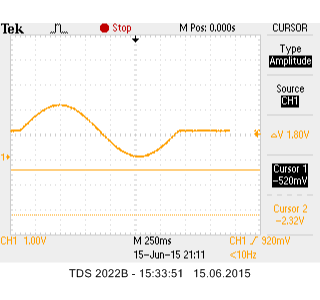
\includegraphics[width=0.7\textwidth]{media/Sinus.png}
	\label{Hoch}
	\caption{Sinussignal}
\end{figure}

\section{Auswertung}
\label{chap:VERSUCH_3_AUSWERTUNG}
Nun messen wir die Zeitdifferenz der einzelnen Stufen mit einer Samplingrate von 10 samples pro Sekunde und erhalten hierdurch eine Zeitdifferenz der einzelnen Stufen von 106 Millisekunden. Dies entspricht einer Frequenz von 10 Hz.
\begin{figure}[H]
	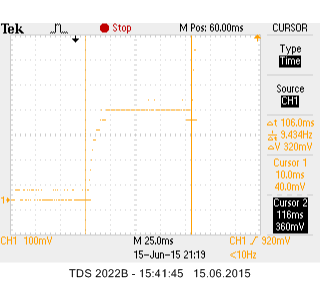
\includegraphics[width=0.7\textwidth]{media/sinus(10samples).png}
	\label{Hoch}
	\caption{Ausschnitt Sinussignal}
\end{figure}

\section{Interpretation}
\label{chap:VERSUCH_3_INTERPRETATION}
Da die Ausgabefrequenz für 10 samples pro Sekunde bei 10 Hz liegt muss die maximale Ausgabefrequenz (100 samples pro Sekunde) bei 100 Hz liegen.
\end{document}